\chapter{Configuration Setup}
%Intro\footnotemark\\
\begin{spacing}{1.2}
%note en bas de page
\section{Configuring the network adapter }

\par In order to configure OpenStack successfully, we will first need to create a network card
Eth0 with the following ip address "10.0.0.30"
\\
\begin{figure}[!htb] 
\begin{center} 
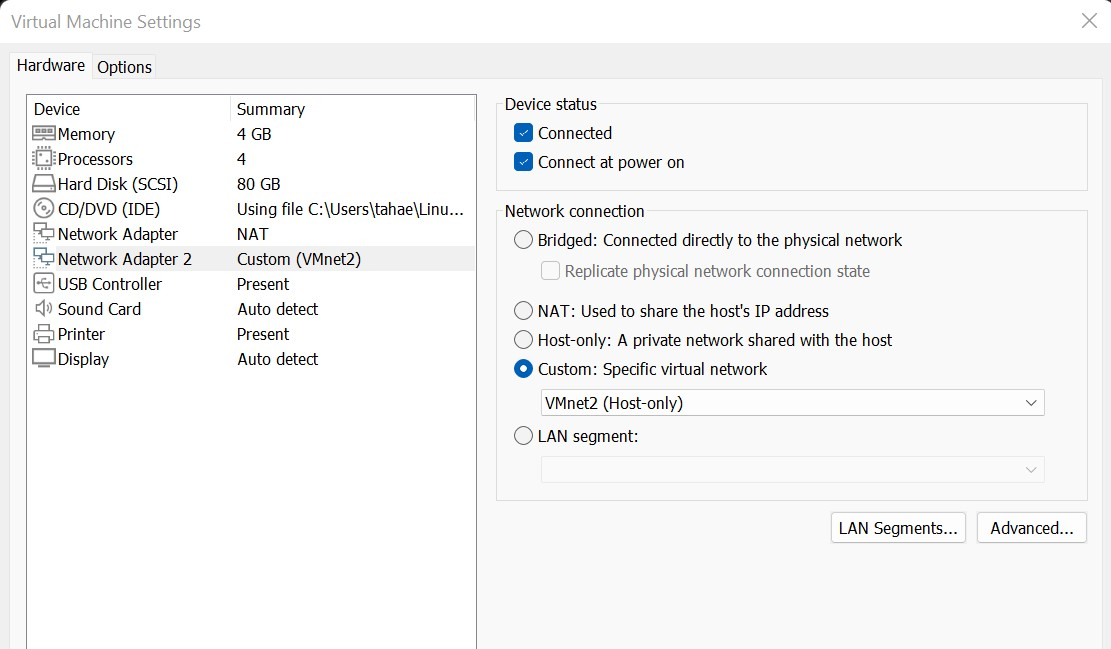
\includegraphics[width=1\linewidth]{Cloud/Config/VM setting} 
\end{center} 
\caption{VM setting} 
\end{figure}  \FloatBarrier
\\
\par In the Virtual Network editor. we are going to modify the new network card created,
for that we will choose the Host-only option, change the Subnet IP / Mask and also change
dhcp parameters as follows: 
\\
\begin{figure}[!htb] 
\begin{center} 
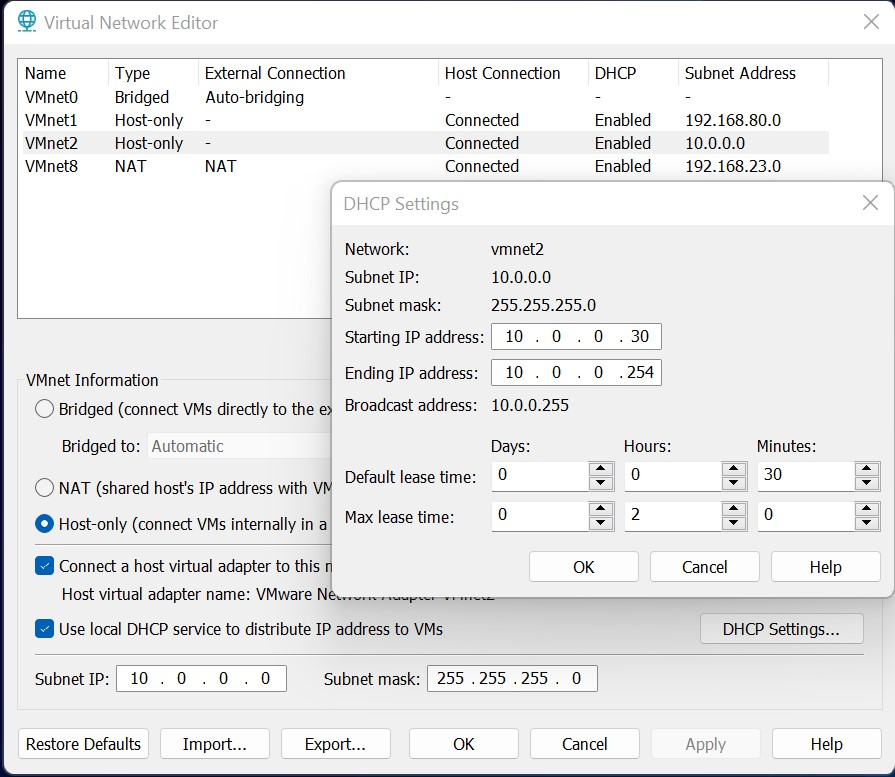
\includegraphics[width=1\linewidth]{Cloud/Config/Virtual Network Editor} 
\end{center} 
\caption{Virtual Network Editor} 
\end{figure}  \FloatBarrier
\\
\section{Installation and configuration of Chrony}

\par Before installing Openstack, you must initially install Chrony in order to configure the NTP server for time synchronization. Next, we will deactivate the firewall because we may causes problems and blocks the installation during this lab.
\\

\begin{figure}[!htb] 
\begin{center} 
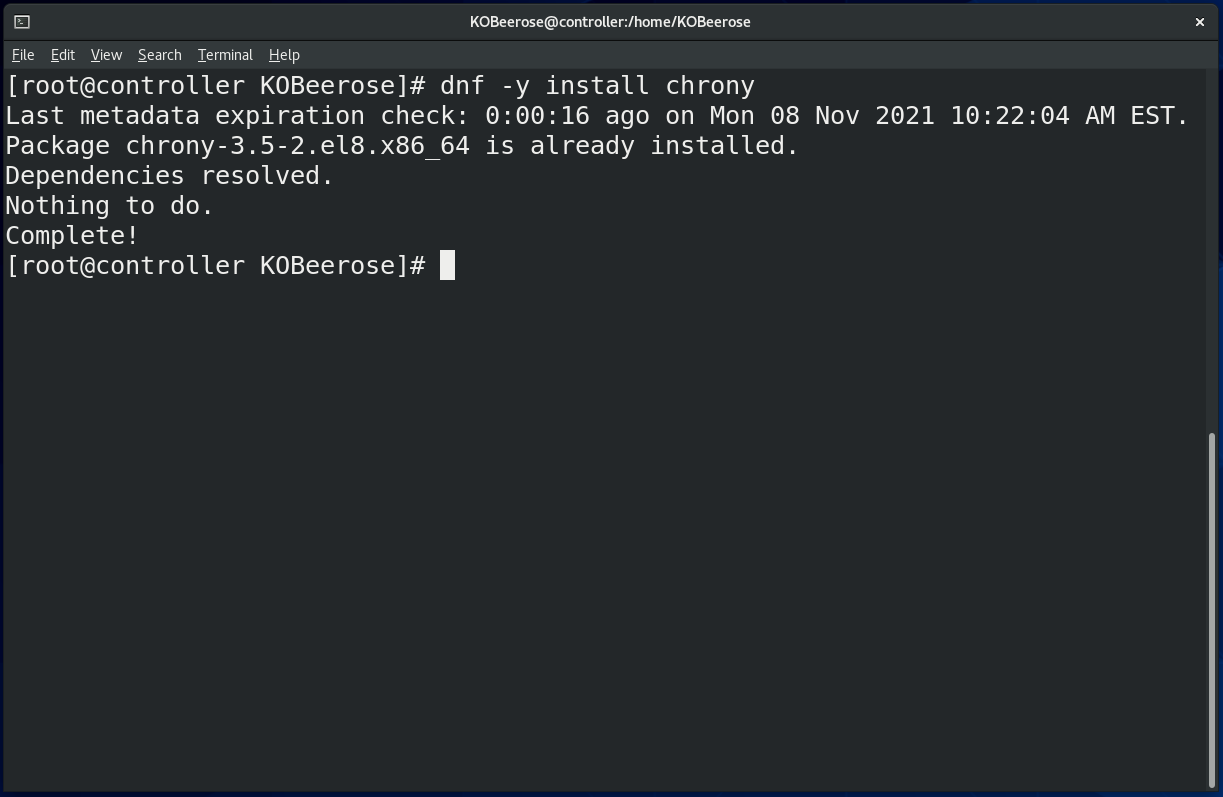
\includegraphics[width=1\linewidth]{Cloud/Config/Installing Chrony} 
\end{center} 
\caption{Installing Chrony} 
\end{figure} \FloatBarrier

\\
\par Also we must add a network range to allow receiving time synchronization requests from NTP clients.
\\
\begin{figure}[!htb] 
\begin{center} 
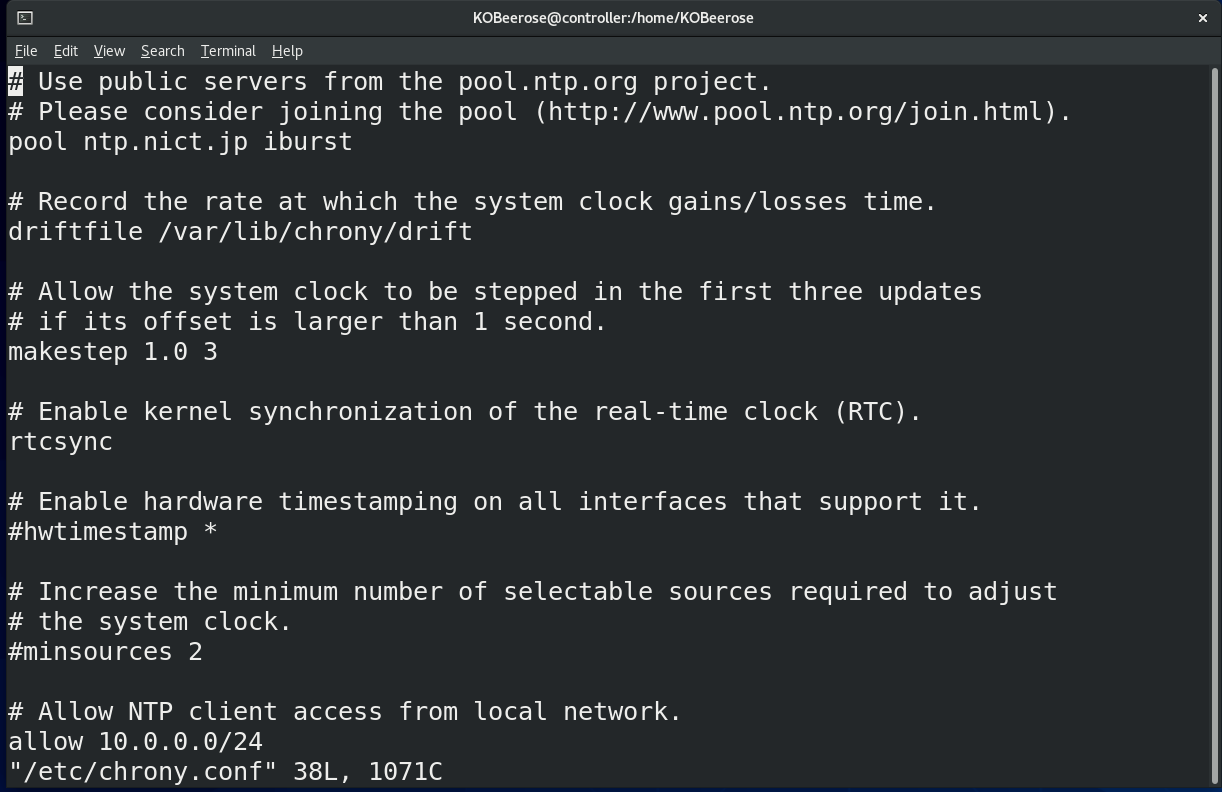
\includegraphics[width=1\linewidth]{Cloud/Config/Changing NTP server} 
\end{center} 
\caption{Changing NTP server} 
\end{figure}  \FloatBarrier
\\


\section{Installation of MariaDB}

\par We will install MariaDB to configure the database server. The installation is launch via the command below, you must then change the Charset which is by default in "Latin" by UTF-8. It is now that mariaDB can be activated.\\

\begin{figure}[!htb] 
\begin{center} 
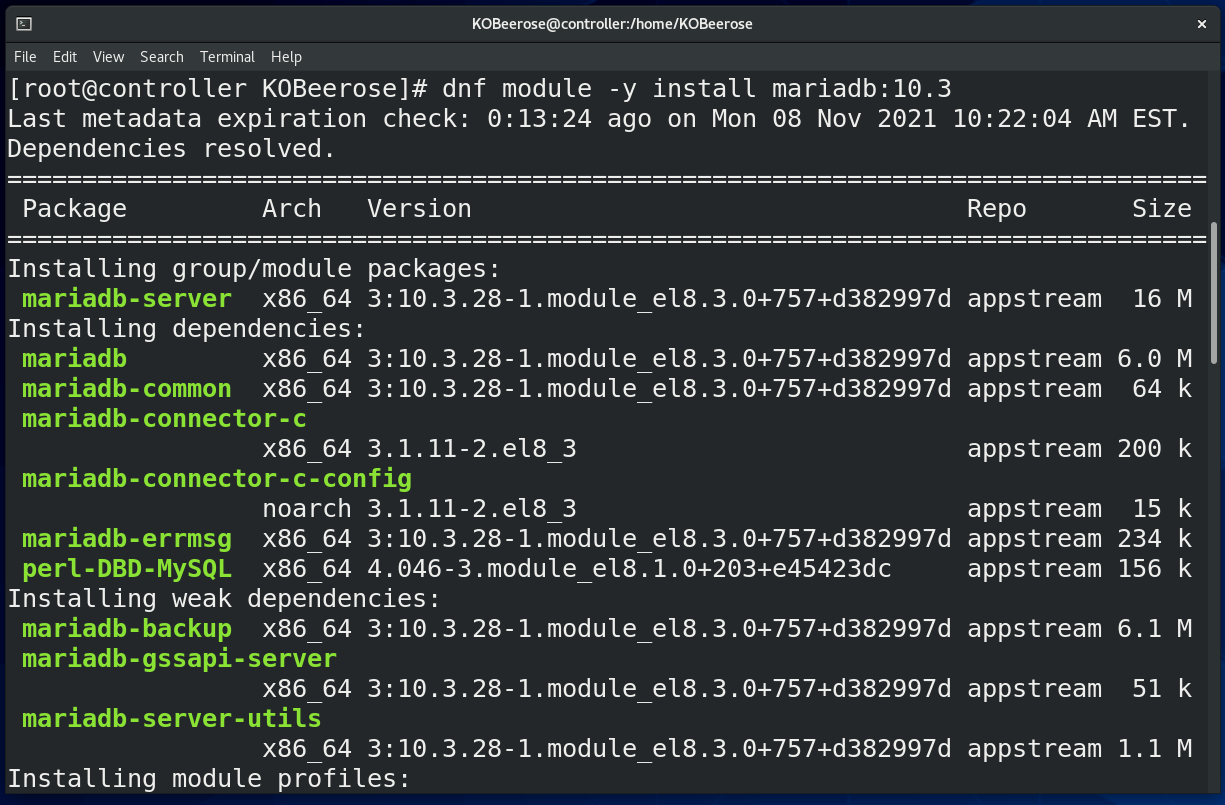
\includegraphics[width=1\linewidth]{Cloud/Config/Installing MariaDB} 
\end{center} 
\caption{Installing MariaDB} 
\end{figure}  \FloatBarrier
\\

\par 
To configure the parameters of MariaDB, we have to execute the command
Mysql secure installation and say yes to all questions. By saying yes, we can define a
password, delete anonymous users, prohibit remote root connection, delete
the test database and reload the privilege tables. 
\\
\begin{figure}[!htb] 
\begin{center} 
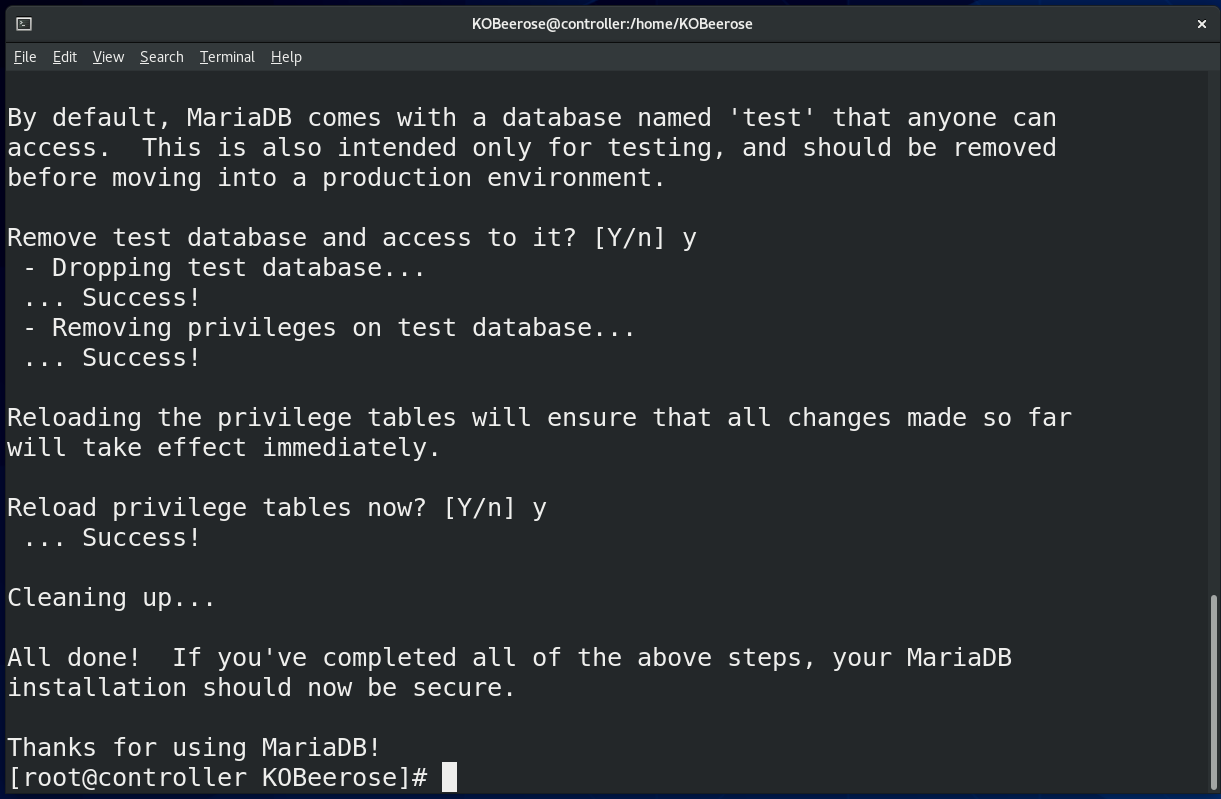
\includegraphics[width=1\linewidth]{Cloud/Config/mysql secure installation} 
\end{center} 
\caption{mysql secure installation} 
\end{figure}  \FloatBarrier
\\


\end{spacing}